\subsection{Optimizers}

A neural network learns to map a set of inputs, \textbf{\textit{X}}, to a corresponding set of outputs, \textbf{\textit{Y}}, while given a subset of correct mappings (training data), $\textbf{\textit{D}}$, where $\textbf{\textit{D}} \subset \textbf{\textit{X}}$, and
% \begin{equation}
%   \begin{aligned}
%     D \subset X
%   \end{aligned}
% \end{equation}
% \begin{equation}
%   \begin{gathered}
%     D = \{(x_i,y_i),...,(x_k,y_k)\}
%   \end{gathered}
% \end{equation}
\begin{center}
$\textbf{\textit{D}} = \{(x_i,y_i),...,(x_k,y_k)\},$
\end{center}
where $(x_i,y_i)$ are individual samples. The network takes the input samples and performs a number of sequential operations to create output estimates, denoted by $\hat y_i$. During the training phase of a neural network, the objective function to be minimized is the derived cost function, $J$, which is remapped to create the loss function $L$, which is dependent on the weights/parameters of the network, $w_i$, as well as $x_i$ (the inputs), $\hat y_i$ (the outputs), and $y_i$ (the correct labels). Thus, training of a neural network can be represented as the optimization problem:

\begin{center}
$\min\limits_{x_i \in X} L(w_i,x_i,y_i,\hat y_i)$
\end{center}

Since the objective function shown above is typically non-convex and can have many pseudo-optimal solutions, direct solutions of the cost function are not feasible. Instead, gradient descent algorithms are used to find these locally minimizing set of parameters using the training data and the corresponding cost/loss function.

In any gradient descent algorithm, a random (or predetermined) initial point, $x_0$, is chosen and then each subsequent value $x_{t+1}$ is determined with the following general updating rule:
\begin{center}
$x_{t+1} = x_t - \eta_t \nabla L_t(w_i,x_i,y_i,\hat y_i) $
\end{center} 
where $\eta_t$ is step length (learning rate), and $\nabla L_t$ is gradient at the current time step. Different algorithms incorporate more variables and calculations into this update step, and/or can add more normalization steps in between updates.

\subsubsection{SGD Algorithm}

The SGD algorithm is one of the most common (and basic) gradient descent algorithms used in the neural network training. The adapted algorithm for mini-batches is as follows:
\vspace{14pt}
\begin{minipage}[b]{.48\textwidth}
\begin{algorithm}[H]\small
	\caption{$Mini-batch\:SGD$ \cite{SGD}}
	\label{alg:SGD}
	\begin{algorithmic}
		\STATE {\bfseries Input:} $x_i \in \mathbb{R}^d$, learning rate $\{\eta_t\}_{t=1}^T$, mini-batch size $B$, $\epsilon>0$
		\vspace{2pt}
		\FOR{$t=1$ {\bfseries to} $T$}
		\vspace{2pt}
		\STATE $G^{(t)}\coloneqq 0$
		\vspace{2pt}
		\FOR{$k=1,...,B$}
		    \vspace{2pt}
		    \STATE Randomly sample point $(\tilde x_k,\tilde y_k)$ from \textbf{\textit{D}}
		    \vspace{2pt}
		    \STATE Compute $\hat y_k$ from current network weights, $w_t$
		    \vspace{2pt}
		    \STATE $G^{(t)}\leftarrow G_k^{(t)} + \frac{1}{B}\nabla L(w_t,\tilde x_{k},\tilde y_k,\hat y_k)$
		    \vspace{4pt}
		\ENDFOR
		\vspace{2pt}
		\STATE $w_{t+1} = w_{t} + \eta_t (G^{(t)} + \epsilon)$
		\vspace{4pt}
		\ENDFOR
	\end{algorithmic}
\end{algorithm}
\end{minipage}\hfill
\vspace{-8pt}

In summary, the mini-batch SGD algorithm states that for every mini-batch (from $1,...,\textit{T}$), the gradient of the loss function will be summed and averaged for each individual sample, $(\tilde x_k,\tilde y_k)$, and the resulting update value $G^{(t)}$ will be used to update the current network weights, $w_i$. The advantage behind performing mini-batches as opposed to weight updates after individual samples is for two reasons:
\vspace{4pt}
\begin{enumerate}
    \item Averaging the gradient across samples has been shown to lower the chances of over-fitting[]
    \item Weight-updates can be performed in a parallel / asynchronous setting, where work can be distributed across individual processors and summed at the end
\end{enumerate}
\vspace{3pt}

Mini-batch SGD has been shown to easily converge many moderately sized neural networks, but fails when the network becomes large or when there is large variance sample to sample.
\subsubsection{LARS optimizer}

The LARS optimizer (short for Layer-wise Adaptive Rate Scaling), developed and outlined by \_ in \cite{ginsburg2018large}, improves upon the previous SGD algorithm by scaling learning rate across individual layers. You et al. found that the ratio of $||w_t||$ ($l_2$ norm of the current weights) to $||g_t||$ (the gradient at the current time step) varied tremendously from the initial to final layers. They propose that scaling the learning rate $\eta_t$ by a second parameter called the "trust" or "lars" coefficient and by the ratio $\frac{||w_t||}{||\nabla L(w_t^l)||}$, training should substantially improve for deep neural networks. They proved this was the case for the ResNet-50 model even when trained with extremely large batch sizes (greater than 32k)\cite{ginsburg2018large}. An outline of the algorithm in the case of SGD with LARS and momentum is as follows:
\begin{minipage}[b]{.48\textwidth}
\begin{algorithm}[H]\small
	\caption{SGD with LARS and momentum \cite{ginsburg2018large}}
	\label{alg:lars}
	\begin{algorithmic}
	    \vspace{3pt}
		\STATE {\bfseries Input:} $x_i \in \mathbb{R}^d$, learning rate $\{\gamma_t\}_{t=1}^T$, $0 < \beta_{1} < 1$ (momentum scaling), LARS coefficient $\eta <1$
		\vspace{3pt}
		\STATE $m_{0} = 0$ (initial momentum term to zero)
		\FOR{$t=1$ {\bfseries to} $T$}
		\vspace{2pt}
		\STATE Randomly sample point $(\tilde x_k,\tilde y_k)$ from \textbf{\textit{D}}
% 		\STATE Draw b samples $S_t$ from $\mathbb{P}$
        \vspace{3pt}
		\STATE $\hat y_k$ (from current network weights, $w_t$)
		\vspace{2pt}
        \STATE $\nabla L(w_t^l,\tilde x_k,\tilde y_k,\hat y_k)$ (gradient at each layer)
        % = \frac{1}{|\mathcal{S}_t|} \sum_{s_t \in \mathcal{S}_t}\nabla \ell(x_t, s_t)$
        \vspace{3pt}
        \STATE $\lambda^l \gets \frac{||w_t^l||}{||\nabla L(w_t^l)||}$ (local LR)
        \vspace{3pt}
        
        \STATE $v_{t} = \beta v_{t-1} + \gamma_t\eta(1 - \beta)\lambda^l\nabla L(w_t^l)$ (momentum calculation)
% 		\STATE $v_{t+1}^l = \eta_t  ||w_t^{(i)}||\frac{m_t^{(i)}}{\|m_t^{(i)}\|} $ for all $i \in [h]$
        \vspace{3pt}
		\STATE $w_{t+1} = w_{t} - v_t$ (update weights)
		\vspace{3pt}
		\ENDFOR
	\end{algorithmic}
\end{algorithm}
\end{minipage}\hfill%
% \begin{algorithm}[htb!]%[t]
% \begin{algorithmic}
% \STATE {\bf Parameters:} base LR $\gamma_0$, momentum $m$, weight decay $\beta$, LARS coefficient $\eta$, number of steps $T$
% \STATE {\bf Init:} $t = 0, v = 0$. Init weight $w_0^l$ for each layer $l$
% \WHILE {$t < T$ for each layer $l$} 
%         \STATE $g_t^l \gets \nabla L(w_t^l)$   (obtain a stochastic gradient for the current mini-batch)
%         \STATE $\gamma_t \gets \gamma_0 * \left(1 - \frac{t}{T}\right)^2$ (compute the global learning rate)
%         \STATE $\lambda^l \gets \frac{||w_t^l||}{||g_t^l|| + \beta ||w_t^l||}$       (compute the local LR  $\lambda^l$)
%         \STATE $v_{t+1}^l \gets mv_t^l + \gamma_{t+1} * \lambda^l * (g_t^l + \beta w_t^l)$     (update the momentum)
%         \STATE $w_{t+1}^l \gets w_t^l - v_{t+1}^l$ (update the 
%         weights)
% \ENDWHILE
% \end{algorithmic}
%  \caption{Mini-batch SGD with LARS. Example with momentum\label{algo:lars}}
% \end{algorithm}

It is important to note that there are two key differences between this implementation and traditional SGD with momentum:
\begin{enumerate}
    \item The learning rate is now parameterized by the layer number, $l$
    \item The calculation of the trust coefficient, $\lambda^l$, is scaled by the LARS coefficient, $\eta$, to apply different magnitudes of LR scaling for each layer
\end{enumerate}
\vspace{4pt}

It can be deduced that dividing by the $l_2$ norms of the loss function and weight vector is effectively normalizing the magnitude of the update step. In practice, this means that only the direction of the gradient is taken into consideration for each update step. It is assumed that this layer-wise normalization allow for deep networks to be trained for higher numbers of iterations with a less likelihood of over-fitting. When applied to the mini-batch case, gradient updates are performed in the same manner, where the gradient updates at each mini-batch are averaged to make a singular update. 

\subsubsection{ADAM optimizer}
Although LARS makes many improvements to traditional SGD algorithms, it still does not incorporate higher-order terms that could benefit each update step. The ADAM optimizer, created by  in \cite{adam}, enhances regular gradient descent algorithms through the addition of two terms and two hyperparameters:
% It introduces exponential moving average on the first and second order of the gradient:
\vspace{-10pt}
\begin{align*}
m_{t} = \beta_{1}m_{t-1}+(1-\beta_{1})g_{t} \\
v_{t} = \beta_{2}v_{t-1}+(1-\beta_{2})g_{t}^2
\end{align*}

The first and second term, $m_{t}$, $v_t$, represent the exponential moving average of the first and second moment of the gradient of the loss function, $g_t$, respectively. The two hyper parameters, $\beta_1$ and $\beta_2$ represent the weighting of the previous and current values. After calculating these two values, there is also a bias correction step:
\begin{align*}
\hat{m}_{t}=\frac{m_t}{1-\beta_1^t} \\
\hat{v}_{t}=\frac{v_t}{1-\beta_2^t}
\end{align*}
\vspace{-10pt}

The addition of these two terms comes from the calculation of the expected value of each moment, which is corrected by dividing the current moment by $(1 - \beta_i^t)$, where t is the current step number. This operation makes $m_t$ and $v_t$ \textit{unbiased estimators} of the first and second moment of the gradient. The algorithm is as follows:
\begin{minipage}[b]{.48\textwidth}
\begin{algorithm}[H]\small
	\caption{ADAM \cite{adam}}
	\label{alg:adam}
	\begin{algorithmic}
		\STATE {\bfseries Input:} $x_i \in \mathbb{R}^d$, learning rate $\{\eta_t\}_{t=1}^T$, parameter $\beta_{1},\beta_{2} \in [0,1)$,  $\epsilon > 0$
		\STATE Initialize $m_{0} = 0, v_{0} = 0$
		\FOR{$t=1$ {\bfseries to} $T$}
		\vspace{2pt}
		\STATE Randomly sample point $(\tilde x_k,\tilde y_k)$ from \textbf{\textit{D}}
		\vspace{2pt}
		\STATE Compute $\hat y_k$ from current network weights, $w_t$
		\vspace{2pt}
		\STATE $g_{t} = \nabla L(w_t,\tilde x_{k},\tilde y_k,\hat y_k)$
		\vspace{2pt}
        \STATE $m_{t} = \beta_{1}m_{t-1}+(1-\beta_{1})g_{t}$
        \vspace{2pt}
        \STATE $v_{t} = \beta_{2}v_{t-1}+(1-\beta_{2})g_{t}^2$
        \vspace{2pt}
        \STATE $\hat{m}_{t}={m_t}/(1-\beta_1^t)$
        \vspace{2pt}
        \STATE $\hat{v}_{t}={v_t}/(1-\beta_2^t)$
        \vspace{2pt}
        \STATE $w_{t+1} = w_{t}-\eta_t\frac{\hat{m}_t}{\hat{v}_t+\epsilon}$
        \vspace{2pt}
		\ENDFOR
	\end{algorithmic}
\end{algorithm}
\end{minipage}\hfill%

\subsubsection{LAMB optimizer}

The LAMB algorithm, developed by \_ in \cite{You2020Large} uses ADAM as the base algorithm, by applies the same layer-wise normalization that LARS implements. More specifically, it makes the following adjustments:
\begin{enumerate}
    \item Using the square root of second moment for normalization
    \item Adopting layer-wise normalization
\end{enumerate}
\begin{minipage}[b]{.5\textwidth}
\begin{algorithm}[H]\small
	\caption{$LAMB$ \cite{You2020Large}}
	\label{alg:lamb}
	\begin{algorithmic}
		\STATE {\bf Input:} $x_1 \in \mathbb{R}^d$, learning rate $\{\eta_t\}_{t=1}^T$,  parameters $0 < \beta_{1}, \beta_2 < 1$, scaling function $\phi$, $\epsilon > 0$
		\STATE Set $m_{0} = 0$, $v_{0} = 0$
		\FOR{$t=1$ {\bf to} $T$}
		\STATE Draw b samples $S_t$ from $\mathbb{P}$.
        \STATE Compute $g_t = \frac{1}{|\mathcal{S}_t|} \sum_{s_t \in \mathcal{S}_t}\nabla \ell(x_t, s_t)$.
		\STATE  $m_{t} = \beta_{1} m_{t-1} + (1 - \beta_{1}) g_{t}$ 
		\STATE  $v_{t} = \beta_{2} v_{t-1} + (1 - \beta_{2}) g_{t}^2$
		\STATE $m_t = m_t/(1 - {\beta}_1^t)$ 
        \STATE $v_t = v_t/(1 - {\beta}_2^t)$
		\STATE Compute ratio $r_t = \frac{m_t}{\sqrt{v_t} + \epsilon}$
		\STATE $x_{t+1}^{(i)} = x_{t}^{(i)} - \eta_t \frac{\phi(\|x_t^{(i)}\|)}{\|r_t^{(i)} + \lambda x_t^{(i)}\|} (r_t^{(i)} + \lambda x_t^{(i)})$
		\ENDFOR
	\end{algorithmic}
\end{algorithm}
\end{minipage}

\subsection{Study Cases' Models}




\subsubsection{Image Classification}

\begin{enumerate}[start=1,label={\bfseries\arabic*:}]
    \item A set of convolution layer and pooling layer to compress the image
    \item Another set of convolution layer and pooling layer to further compress the data
    \item Two fully connected layers after flattens the data to do the neural network training.
    \end{enumerate}
    
%The first part of the network is a straightforward CNN model and it uses Relu as activation function. It consists of two consecutive convolution layer and pooling layer in order to capture the potential features of the images. The second part of the network flattens the condensed image and then uses two fully connected layer to do the classification.

The cost function is calculated by negative log likelihood loss:
\begin{align*}
    J(y) = -log(y) 
\end{align*}

Note there is only one term in the loss function per data, which is the negative log likelihood of the predicted value of the true label. This negative loss likelihood function works better when the neural network model has a high confidence at the correct class. When training in batch, the cost function per batch is the sum of the individual negative log likelihood costs.

\subsubsection{QA System}


The model employed for QA understanding system here is called Document retriever Question Answering (DrQA) as illustrated in Figure~\ref{fig:DrQA}.  Starting from the top:
\begin{enumerate}[start=1,label={\bfseries\arabic*:}]
    \item According to Lee et al. \cite{Lee}, the questions and context can be aligned to build respective embedding of: 
    \begin{center} $f_{align} = \sum_j \alpha_{i, j} E(q_j)$. \end{center}
    
    Where $\alpha$ is single dense layer with relu non-linearity and $E()$ represents the glove embeddings. This layer help initialize what portion of the context is more important or relevant with respect to the question.
    
    \item In order to understand the representation of these glove and aligned paragraphs, these are passed to stacked bi-LSTM \cite{biLSTM}. LSTM is expressed as: 
    \begin{center}
    $u_t = \sigma(W_u x_t + U_u h_{t-1} + b_u)$ \\
    $f_t = \sigma(W_f x_t + U_f h_{t-1} + b_f)$  \\
    $g_t = tanh(W_g x_t + U_g h_{t-1} + b_g)$  \\
    $o_t = \sigma(W_o x_t + U_o h_{t-1} + b_o)$  \\
    $c_t = f_t c_{t-1} + u_t g_t$ \\
    $h_t = o_t tanh(c_t)$
    \end{center}
    
    where $u, f, g, o$ are  respectively update/input, forget, cell, and output gates. $c_t$ is the cell at time $t$ and $\sigma(\cdot)$ is the sigmoid function. 
    
    \item Then the importance of each word in the question is calculated through Linear Attention layer as $b$ below with $w$ as a trainable weight vector:
    \begin{center} 
    $b_j = \frac{e^{w \cdot q_j}}{\sum_{j'}e^{w\cdot q_{j'}}}$
    \end{center}
    
    \item Finally, to predict the accurate answer's span tokens, there are two bilinear classifiers to respectively predict the probabilities of start and end tokens of the span: 
    \begin{center} 
    $P_{start}(i) \propto e^{p_iW_sq}$ \\
    $P_{end}(i) \propto e^{p_iW_eq}$
    \end{center}
    
    
\end{enumerate}


\begin{figure}[!t]
    \centering
    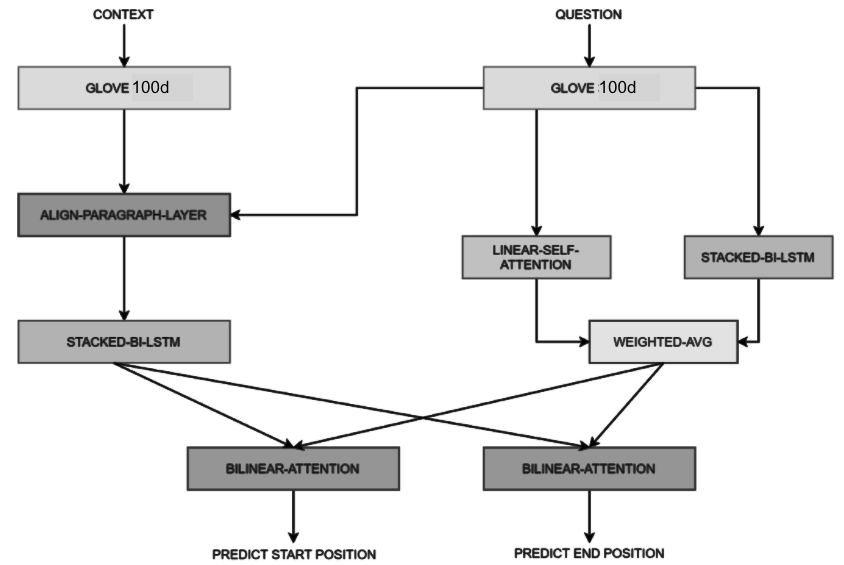
\includegraphics[width=\linewidth]{img/DrQA.png}
    \caption{Document Reader model architecture part of DrQA \cite{DrQA}}
    \label{fig:DrQA}
\end{figure}

% As the name suggested, the model included Document Retriever and Document Reader: 




\subsubsection{Speech to Text}

The model is a variant of the Deep Speech 2 model with the aid of Residual CNN (Res-CNN)

% Model is similar to Deep Speech 2, model, but first preprocesses the data into a spectrogram, then these are fed into 3 Residual CNN blocks to extract feature vectors of length 500 from the audio data, and a set of 3 bidirectional GRU-RNN layers to translate the extracted features into an intermediate output vector, which is fed into a fully connected layer, then a softmax, then a 28 long vector mapping of probabilities of corresponding letters or symbols.

\begin{figure*}[!t]
    \centering
    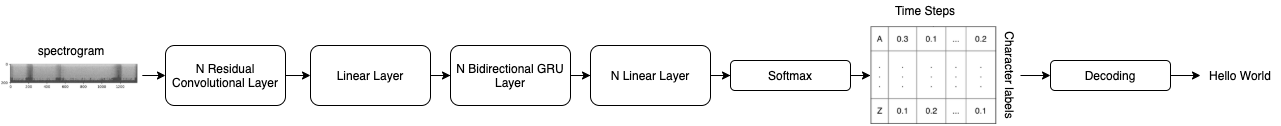
\includegraphics[width=\linewidth]{img/speech.png}
    \caption{A variant of Deep Speech 2 architecture that utilizes Res-CNN.}
    \label{fig:deepSpeech}
    \vspace{-10pt}
\end{figure*}

\begin{enumerate}[start=1,label={\bfseries \arabic*:}]
    \item Residual network consists of stacked ``residual units'' inspired by He et al. \cite{resnet} but with layer norm to learn the audio features expressed as:
    \begin{center}
    $x_{l + 1} = ReLU(h(x_l) + F(x_l, W_l))$ \\
    \end{center}
    
    \item A fully connected layer to compress the model representation before passing it over. 
    
    \item Bidirectional GRU-RNN \cite{biGRURNN} is then utilized to leverage the features to learn the representation of the audio's spectrogram frames before the current step and after it as well. 
    
    \begin{center}
    
    $u_t &= \sigma(W_u x_t + U_u h_{t-1} + b_u)$ \\
    $r_t &= \sigma(W_r x_t + U_r h_{t-1} + b_r)$ \\
    $\tilde{h}_t &= f(W_h x_t + r_t \circ U_h h_{t-1} + b_h)$ \\
    $h_t &= (1 - u_t) h_{t-1} + u_t \tilde{h}_t$

    \end{center}
    
    $u$ and $r$ represent the \emph{update} and \emph{reset} gates respectively. This is slightly different from the standard GRU in that the hidden state $h_{t-1}$ is multiplied by $U_h$ prior to scaling by the reset gate. This allows for all operations on $h_{t-1}$ to be computed in a single matrix multiplication. Moreover, Amodei et al. \cite{Amodei} found similar performance for $tanh$ and clipped-ReLU for nonlinear transformation so clipped-ReLU \cite{clippedReLU} is picked for simplicity and uniformity with the rest of the network.

    
    \item A final fully connected layer takes the inputs from the feature analysis and applies weights to predict the correct label.
    
    \item A Gaussian Error Linear Unit (GELU) activation layer as: 
    
    \begin{center}
    $GELU(x) = xP(X \leq x) = x \cdot \frac{1}{2} [1 + erf(\frac{x}{\sqrt{2}}]$
    \end{center}
    
    \item A linear layer to map the results to final probabilities for each mapping of corresponding letters or symbols. 
    
\end{enumerate}

